%\documentclass[wcp,gray]{jmlr} % test grayscale version
\documentclass[wcp]{jmlr}

% The following packages will be automatically loaded:
% amsmath, amssymb, natbib, graphicx, url, algorithm2e

%\usepackage{rotating}% for sideways figures and tables
\usepackage{longtable}% for long tables

% The booktabs package is used by this sample document
% (it provides \toprule, \midrule and \bottomrule).
% Remove the next line if you don't require it.
\usepackage{booktabs}
% The siunitx package is used by this sample document
% to align numbers in a column by their decimal point.
% Remove the next line if you don't require it.
%\usepackage[load-configurations=version-1]{siunitx} % newer version
%\usepackage{siunitx}

% The following command is just for this sample document:
\newcommand{\cs}[1]{\texttt{\char`\\#1}}

% This is required for dmath (display math)
\usepackage{breqn}

\jmlrvolume{29}
\jmlryear{2013}
\jmlrworkshop{ACML 2013}

\title[MML Laplace]{Minimum Message Length Inference of Laplace Distribution}

 % Use \Name{Author Name} to specify the name.
 % If the surname contains spaces, enclose the surname
 % in braces, e.g. \Name{John {Smith Jones}} similarly
 % if the name has a "von" part, e.g \Name{Jane {de Winter}}.
 % If the first letter in the forenames is a diacritic
 % enclose the diacritic in braces, e.g. \Name{{\'E}louise Smith}

 % Two authors with the same address
 % \author{\Name{Author Name1} \Email{abc@sample.com}\and
 %  \Name{Author Name2} \Email{xyz@sample.com}\\
 %  \addr Address}

 % Three or more authors with the same address:
 % \author{\Name{Author Name1} \Email{an1@sample.com}\\
 %  \Name{Author Name2} \Email{an2@sample.com}\\
 %  \Name{Author Name3} \Email{an3@sample.com}\\
 %  \Name{Author Name4} \Email{an4@sample.com}\\
 %  \Name{Author Name5} \Email{an5@sample.com}\\
 %  \Name{Author Name6} \Email{an6@sample.com}\\
 %  \Name{Author Name7} \Email{an7@sample.com}\\
 %  \Name{Author Name8} \Email{an8@sample.com}\\
 %  \Name{Author Name9} \Email{an9@sample.com}\\
 %  \Name{Author Name10} \Email{an10@sample.com}\\
 %  \Name{Author Name11} \Email{an11@sample.com}\\
 %  \Name{Author Name12} \Email{an12@sample.com}\\
 %  \Name{Author Name13} \Email{an13@sample.com}\\
 %  \Name{Author Name14} \Email{an14@sample.com}\\
 %  \addr Address}


 % Authors with different addresses:
  \author{\Name{Author Name1} \Email{abc@sample.com}\\
  \addr Address 1
  \AND
  \Name{Author Name2} \Email{xyz@sample.com}\\
  \addr Address 2
 }

\editor{Cheng Soon Ong and Tu Bao Ho}
% \editors{List of editors' names}

\begin{document}

\maketitle

\begin{abstract}
This paper aims at bringing out the merits of using the Laplace distribution over
the Normal distribution. The choice of the best distribution is objectively
made using the minimum message length (MML) principle. The message length for
transmitting data using a Laplace distribution is derived and its parameters are
estimated. This method of transmission is compared with that of transmistting the data
using the Normal distribution. This is explored in the context of superposition
of protein structures. The optimal superposition of protein structures (described
using a Normal distribution) minimizing the L2 norm is computed using the 
Kearsley's method and the superposition minimizing the
L1 norm (described using a Laplace model) is approximated using Monte Carlo 
simulation. These two are compared with respect
to their model complexity and the overall fit to the data using MML. 
\end{abstract}

\begin{keywords}
Laplace, Normal, MML, Kearsley, Monte Carlo simulation
\end{keywords}

\section{Introduction}
Normal distribution is widely used in modelling a set of data whose true distribution
is unknown. In many problems, the objective function is formulated as a sum of squares,
(the L2 norm) and this function is minimized or maximized depending on the application. 
Normal distribution has a huge impact on the cost function because of the squared nature of 
the individual terms. If there are outliers in the dataset, the final inference might be 
skewed to accommodate the outliers in the model description. The Laplace distribution, 
however, is robust to
outliers as the objective function involves the sum of the absolute values of the difference 
of the individual terms (L1 norm).
The choice of selecting a Laplace over Normal is investigated in this paper. This
selection is made by formulating the objective function using Minimum Message
Length (MML). The distribution which results in the best compression of data is chosen
to be the best model. \\

Normal distribution is expressed in terms of squared difference from the mean $\mu$
\eqref{eqn:normal_pdf},
\begin{equation}
\mathrm{pdf}(x) = \frac{1}{\sqrt{2\pi\sigma}} \mathrm{exp}\left(-\frac{(x-\mu)^2}{2\sigma^2}\right) \label{eqn:normal_pdf}
\end{equation}
and hence objective functions based on minimizing the total least squares result in a 
closed form analytical solution. On the contrary, because of the mathematical
nature of the Laplace \eqref{eqn:laplace_pdf} which is expressed as the absolute 
difference from the mean, does not offer a closed form solution.
\begin{equation}
\mathrm{pdf}(x) = \frac{1}{2b}\mathrm{exp}\left(-\frac{|x-\mu|}{b}\right) \label{eqn:laplace_pdf}
\end{equation}
That being said, we however, believe that it has potential benefits. Laplace distribution
is a model of choice in areas as diverse as signal processing 
\citep{laplace-signal-processing}, image denoising \citep{image-denoising},
gene expression studies \citep{Bhowmick01102006}, market risk prediction
\citep{haas2005modeling}, and machine learning \citep{Cord:2006:FSR:1167556.1167570}.
In most of these applications, a mixture model of Laplace distributions is used. \\

The main contribution of this work is the derivation of the message length 
expression and estimation of the MML parameters for the Laplace distribution.
The general procedure to formulate the message length expression for transmitting
data using some statistical model is outlined in \citet{wallace-87}. The MML method
of estimating parameters for a number of distributions has been well established
\citep{WallaceBook}. This general approach is followed in the derivation of the
message length expression for the Laplace distribution. \\

We demonstrate its use in two cases. The first scenario involves data being randomly
generated from an underlying Laplace distribution. This data is then fitted using
both Normal and Laplace models. We use the derived formulation of MML for modelling
the data using Laplace distribution. It is observed that the compression in message
length is better when compared to transmitting it over a Normal distribution. Since
the original distribution from which the data was generated happens to be Laplace,
it is reasonable to guess that a Laplace model fits better. In general, if the
data is generated from an underlying true distribution, modelling that data using
the same statistical model results in a better fit.
This is done as a validation check to ensure that the MML formulation for the 
Laplace case is consistent with this observation. \\

Further, we demonstrate its use by applying to the problem of optimal superposition.
Examples of protein structures are considered
and they are superposed using Kearsley's transformation. This results in an
orientation of the proteins which minimizes the total least squares deviations. 
This optimal superposition is then encoded using a Normal distribution.
A related superposition which minimizes the total absolute 
value of the deviations is then computed using a Monte Carlo 
simulation. This optimal superposition is encoded using a Laplace distribution.

\section{The Minimum Message Length (MML) Framework}
\subsection{Inductive Inference}
\citet{wallace68} developed the first practical criterion for model selection using 
information theory. MML provides an elegant framework to compare any two competing 
hypotheses that model some observed data. The hypothesis that results in the shortest 
overall message length is chosen as the best one, in line with traditional statistical 
inference using the Bayesian method.\footnote{http://allisons.org/ll/MML/} \\

Using Bayes' theorem to explain some observed data $D$ by hypothesis $H$, we get:
\begin{equation*}
  \Pr(H\&D) = \Pr(H) \times \Pr(D|H) = \Pr(D) \times \Pr(H|D)
\end{equation*}
where $\Pr(H\&D)$ is the joint probability of data $D$ and hypothesis $H$. $\Pr(H)$
is the prior probability of hypothesis $H$, $\Pr(D)$ is the prior probability of 
probability of data $D$, $\Pr(H|D)$ is the posterior probability of $H$
given $D$, and $\Pr(D|H)$ is the likelihood.
MML uses the following result from information theory: given an event $E$
with a probability $\Pr(E)$, the message length $I(E)$ for an optimal
code is given by $I(E) = -\log_2 (\Pr(E))$ bits \citep{shannon1948}. Applying this insight
to the Bayes' theorem, we get the following relationship between
conditional probabilities in terms of optimal message lengths:
\begin{equation*}
  I(H\&D) = I(H) + I(D|H) = I(D) + I(H|D)
\end{equation*}
In the traditional Bayesian framework, the hypothesis $H$ with
the largest posterior probability $\Pr(H|D)$ is often preferred.
Among the terms in the above equation, $\Pr(H)$ (and hence $I(H)$) can
usually be estimated well for \emph{some} reasonable prior(s) on hypotheses.
Given the data $D$ and a chosen prior $H$, the likelihood $\Pr(D|H)$ can also be estimated.
Whilst comparing two competing hypotheses, the prior of observed data $\Pr(D)$
can be ignored as it is a common factor. Hence, for two competing hypotheses, $H$ and $H^\prime$, we have:
\begin{equation*}
I(H|D) - I(H^\prime|D) = I(H) + I(D|H) - I(H^\prime) - I(D|H^\prime)
\end{equation*}
The message, therefore, comprises of two parts: 
\begin{enumerate}
\item Statement of the hypothesis $H$ (given by $I(H)$)  
\item Statement of the data $D$ using the hypothesis (given by $I(D|H)$) 
\end{enumerate}

\subsection{Parameter Estimation using MML}
The hypothesis is a statistical model which is characterized by a set of parameters.
MML treats the parameters and data as entities which need to be passed on as 
information by a transmitter to a receiver. There is a message length associated
with encoding both the parameters and the data. The main difference between MML and
other Bayesian methods of inference is in the importance they give to the
parameters of the model. As an example, most methods based on manimum likelihood (ML)
ignore the prior distribution of the parameters. In the MML approach, both the 
parameters and the data are stated to some precision. The message length varies
with the precision. If the parameters are stated more accurately than required, the 
message length might be longer although this might lead to a better fit to the data. 
MML works by identifying the precision to which these 
parameters need to be stated. \citet{wallace-87} provide an approximation to infer
these precision values which balance the tradeoff of precision of parameters and the 
fit to the data. Such an elegant way allows us to compare two hypotheses which
model the same data but using different sets of parameters.

\section{Message Lengths of Normal \& Laplace distributions}
\citet{wallace-87} derived the code length of the two part message as
\begin{align}
I(\bar{\theta},D) &= I(\bar{\theta}) + I(D|\bar{\theta}) \notag\\
&\approx \underbrace{\frac{d}{2}\log\kappa_d -\log h(\bar{\theta}) + \frac{1}{2}\log(det\,F(\bar{\theta}))}_{\mathrm{part 1}} + \underbrace{L(\bar{\theta}) + \frac{d}{2}}_{\mathrm{part 2}} \label{eqn:wf_msglen}
\end{align}
where $\bar{\theta}$ is the set of model parameters, $d$ is the number of parameters, 
$\kappa_d$ is the $d$-dimensional lattice quantization constant \citep{conwaySloane84}, 
$h(\bar{\theta})$ is the prior probability of the parameters, 
$det(\mathrm{F}(\bar{\theta}))$ is the determinant of the expected Fisher matrix, and
$L(\bar{\theta})$ is the negative log likelihood of observed data. The MML estimates 
$\hat{\bar{\theta}}_{\mathrm{MML}}$ of the parameters are determined by minimizing 
\eqref{eqn:wf_msglen}. 

\subsection{Normal distribution}
The parameters describing the Normal distribution \eqref{eqn:normal_pdf} are the mean $\mu$
and the standard deviation $\sigma$. Let $D = \{x_1,x_2,\ldots,x_N\}$ be the observed data 
containing $N$ samples, $\epsilon$ be the precision to which each datum is stated. 
Let $\mathrm{R}_{\mu}$, $\mathrm{R}_{\sigma}$ be the range of $\mu$ and $\log\sigma$ 
respectively. $\epsilon$, $\mathrm{R}_{\mu}$, $\mathrm{R}_{\sigma}$ are hyperparameters
which are introduced in \citet{WallaceBook}. The derivation of the MML estimates 
for a Normal distribution is presented in \citet{WallaceBook}. The MML estimates are:
\begin{align*}
\hat{\mu}_{\mathrm{MML}} &= \frac{1}{N} \sum_{n=1}^N x_n \\
\hat{\sigma}_{\mathrm{MML}} &= \sqrt{\frac{1}{N-1} \sum_{n=1}^N (x_n-\hat{\mu}_{\mathrm{MML}})^2}
\end{align*}
The corresponding minimized message length is given as
\begin{dmath}
 \therefore I_{min} = I(\hat{\mu}_{\mathrm{MML}},\hat{\sigma}_{\mathrm{MML}}) = 1 + \log\kappa_2 + \log(\mathrm{R}_{\mu}\mathrm{R}_{\sigma}) + \frac{1}{2}\log(2N^2) + \frac{N}{2}\log\left(\frac{2\pi}{\epsilon^2}\right) + \frac{N-1}{2}\log\left(\frac{\sum_{n=1}^N (x_n-\hat{\mu}_{\mathrm{MML}})^2}{N-1}\right) + \frac{N-1}{2}  \label{eqn:normal_mml_estimate}
\end{dmath} 

\subsection{Laplace distribution}
The novelty of this paper lies in the derivation of the MML estimates of 
the parameters of the Laplace distribution.
The parameters describing a Laplace distribution are the $\mu$ and $b$. $\mu$ 
is the mean of the distribution and $b$ is the scale parameter. The probability
density function is given in \eqref{eqn:laplace_pdf}. To derive these estimates,
we use the Wallace-Freeman approximation \citep{wallace-87}. This requires:
\begin{itemize}
  \item a likelihood function
  \item the Fisher information matrix
  \item prior distributions on the parameters
\end{itemize}
Using \eqref{eqn:laplace_pdf}, the \emph{likelihood function} is
\[ f(D|\bar{\theta}) = \prod_{n=1}^N \frac{\epsilon}{2b} e^{-\frac{|x_n-\mu|}{b}} \]
and hence the \emph{negative log-likelihood} is computed as
\begin{align}
 L(\bar{\theta}) &= -\log f(D|\bar{\theta}) \notag\\
		 &= N\log\left(\frac{2}{\epsilon}\right) + N\log b + \frac{1}{b}\sum_{n=1}^N |x_n-\mu| \label{eqn:laplace_l}
\end{align}
The maximum likelihood (ML) estimates for $\mu$ and $b$ are given by
\begin{align*}
\hat{\mu}_{\mathrm{ML}} &= \mathrm{median}\{x_n\} \\ 
\hat{b}_{\mathrm{ML}} &= \frac{1}{N} \sum_{n=1}^N |x_n-\hat{\mu}_{\mathrm{ML}}|
\end{align*}

\subsection*{Computation of Fisher information $\mathbf{F(\bar{\boldsymbol{\theta}})}$}
The Fisher information matrix is given by
\begin{align*}
  \mathrm{F}(\mu,b) &= \left( \begin{array}{cc}
  \mathrm{E} \left[\frac{\partial^2 L}{\partial \mu^2}\right] & \mathrm{E} \left[\frac{\partial^2 L}{\partial\mu \partial b}\right] \\
  \mathrm{E} \left[\frac{\partial^2 L}{\partial b \partial\mu}\right] & \mathrm{E} \left[\frac{\partial^2 L}{\partial b^2}\right] 
  \end{array} \right) 
\end{align*}
where $\mathrm{E}[.]$ is the expected value of that quantity. Using \eqref{eqn:laplace_l},
\begin{align*}
 \frac{\partial^2 L}{\partial b^2} &= -\frac{N}{b^2} + \frac{2}{b^3} \sum_{n=1}^N |x_n-\mu| \\
 \mathrm{E} \left[\frac{\partial^2 L}{\partial b^2}\right] &= -\frac{N}{b^2} + \frac{2}{b^3} \mathrm{E}\left[\sum_{n=1}^N |x_n-\mu|\right]
\end{align*}
\begin{align*}
 \mathrm{E}\left[|x-\mu|\right] &= \int\limits_{-\infty}^{\infty} |x-\mu| . \frac{1}{2b} . e^{-\frac{|x-\mu|}{b}} dx \\
 &= \frac{1}{2b} \int\limits_{-\infty}^{\mu} -(x-\mu) e^{\frac{(x-\mu)}{b}} dx + \int\limits_{\mu}^{\infty} (x-\mu)e^{-\frac{(x-\mu)}{b}} dx \\
 &= b
\end{align*}
\begin{equation*}
 \therefore \mathrm{E} \left[\frac{\partial^2 L}{\partial b^2}\right] = -\frac{N}{b^2} + \frac{2}{b^3} (Nb) = \frac{N}{b^2} 
\end{equation*}
The computation of $\mathrm{E}\left[\frac{\partial^2 L}{\partial \mu^2}\right]$ and 
$\mathrm{E}\left[\frac{\partial^2 L}{\partial \mu \partial b}\right]$ is involved and hence,
tucked away in \autoref{apd:laplace_fisher}. Using those results, we have
\begin{align*}
  \mathrm{F}(\mu,b) &= \left( \begin{array}{cc}
        \frac{N}{b^2} & 0 \\
        0 & \frac{N}{b^2}
            \end{array} \right) 
\end{align*}
\begin{equation} \therefore det(\mathrm{F}(\mu,b)) = \frac{N^2}{b^4} \label{eqn:laplace_fisher} \end{equation}

\subsection*{Priors on the parameters}
A prior probability on $\mu$ and $b$ is assumed in accordance with the prior assumed
in the case of Normal. The ranges from which $\mu$ and $\log b$ are drawn are prespecified as 
$\mathrm{R}_{\mu}$ and $\mathrm{R}_{b}$ respectively \citep{WallaceBook}. 
\begin{align} 
\therefore h(\bar{\theta}) = h(\mu,b) &= h(\mu) h(b) \notag\\
      &= \frac{1}{\mathrm{R}_{\mu}}. \frac{1}{b \mathrm{R}_{b}} \label{eqn:laplace_h} 
\end{align}

Using \eqref{eqn:wf_msglen}, \eqref{eqn:laplace_fisher}, \eqref{eqn:laplace_h},
\begin{dmath*}
 I(\mu,b) = \left( \log\kappa_2 + \log(\mathrm{R}_{\mu}\mathrm{R}_{\sigma}) + \log N - \log b \right) + \left( N\log\left(\frac{2}{\epsilon}\right) + N\log b + \frac{1}{b}\sum_{n=1}^N |x_n-\mu| + 1 \right)
\end{dmath*} 

\noindent To obtain the MML estimates $\hat{\mu}_{\mathrm{MML}}$ and $\hat{b}_{\mathrm{MML}}$ 
which results in minimum $I$, $\frac{\partial I}{\partial \mu} = 0$ and 
$\frac{\partial I}{\partial b} = 0$. The MML estimates are therefore, given by
\begin{align}
  \hat{\mu}_{\mathrm{MML}} &= \mathrm{median}\{x_n\} \notag\\
  \hat{b}_{\mathrm{MML}} &= \frac{1}{N-1} \sum_{n=1}^N |x_n-\hat{\mu}_{\mathrm{MML}}| 
  \label{eqn:laplace_estimate}
\end{align}
The corresponding minimized message length is given as
\begin{dmath}
 \therefore I_{min} = I(\hat{\mu}_{\mathrm{MML}},\hat{b}_{\mathrm{MML}}) = 1 + \log\kappa_2 + \log(\mathrm{R}_{\mu}\mathrm{R}_{\sigma}) + \log N + N\log\left(\frac{2}{\epsilon}\right) + (N-1) \log \left( \frac{\sum_{n=1}^N |x_n-\hat{\mu}_{\mathrm{MML}}|}{N-1} \right) + (N-1) \label{eqn:laplace_mml_estimate}
\end{dmath} 

\section{Experiments}
We demonstrate the use of Laplace estimates in two scenarios. 

\subsection{Data generation and modelling}
In the first case, data is generated randomly from a distribution (Normal \& Laplace) 
separately. This data is then modelled using the two distributions.
It is observed that if the true distribution is a Laplace, then it is better
modelled by a Laplace. \eqref{eqn:laplace_mml_estimate} is used to determine
the code length when the data is modelled using the Laplace distribution.
\eqref{eqn:normal_mml_estimate} is used to encode the data using a Normal
distribution. \\

As an example, 500 random samples are generated from each of the distributions.
The mean of the true distribution is taken to be 0 and the spread (standard
deviation $\sigma$ for a Normal and scale parameter $b$ for a Laplace) is
chosen to be 2. \autoref{fig:data_approximation} shows the original distributions
and the corresponding Normal and Laplace approximations. In \autoref{fig:normal_data},
the true distribution is normal (red curve). The Normal approximation (blue curve)
overlaps almost entirely with the red curve which is an indication of a good fit.
The Laplace approximation (green curve) significantly deviates from the original
distribution. The same argument holds for \autoref{fig:laplace_data} where the
underlying distribution of the data is Laplace, and hence, in this case, the Laplace
seems to be a good fit. \\

\autoref{tab:comparison_estimates} provides a comparison of the estimates of the
two distributions. The message length (msglen) is computed in bits. It can be seen
when the true distribution is Laplace, the message length corresponding to the Laplace 
estimate (6690.91 bits) is smaller compared to that of the Normal estimate (6755.68 bits).

\begin{figure}[!htb]
  \centering
    \subfigure[Original distribution: Normal]
    {
      \centering
        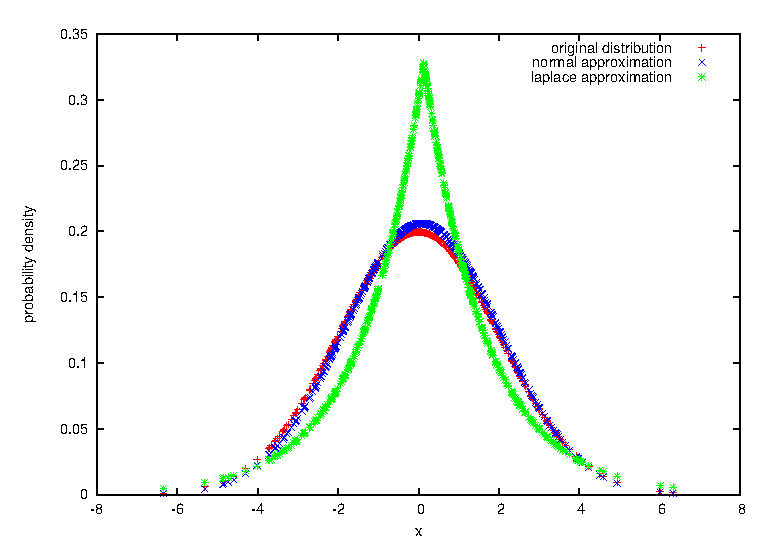
\includegraphics[width=0.45\textwidth]{fig/normal_n_500_mean_0_scale_2.eps}
        \label{fig:normal_data}
    }
    \hspace{0.5cm}
    \subfigure[Original distribution: Laplace]
    {
        \centering
        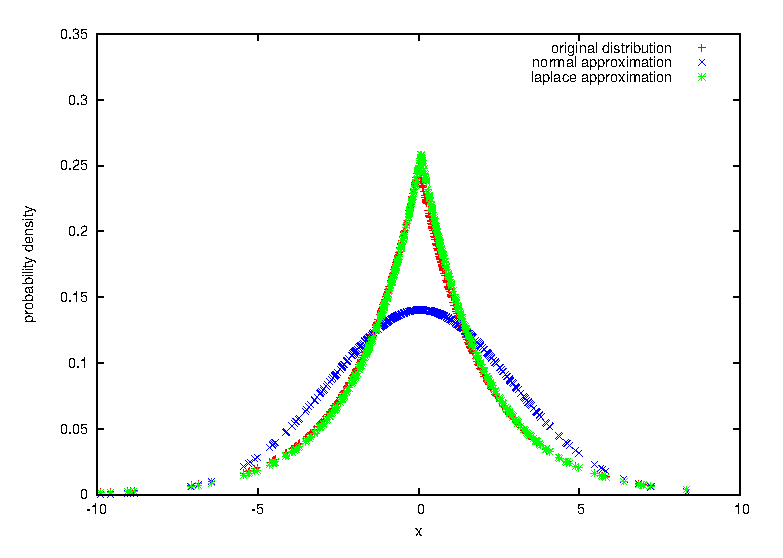
\includegraphics[width=0.45\textwidth]{fig/laplace_n_500_mean_0_scale_2.eps}
        \label{fig:laplace_data}
    }
    \caption{Approximation of data using Normal \& Laplace distributions}
    \label{fig:data_approximation}
\end{figure}

\begin{table}[h]
\centering
\caption{Comparison of the estimates}
\label{tab:comparison_estimates}
\begin{tabular}{|c|c|c|c|c|c|c|c|c|}
\hline
True & True & True & \multicolumn{3}{c|}{Normal estimates} & \multicolumn{3}{c|}{Laplace estimates} \\ \cline{4-9} 
distribution & mean & spread & mean & spread & msglen & mean & spread & msglen \\ \hline 
Normal & 0 & 2 & 0.0722611 & 1.93638 & 6493.89 & 0.127191 & 1.52389 & 6518 \\ \hline
Laplace & 0 & 2 & -0.0455104 & 2.78563 & 6755.68 & 0.0471194 & 1.9376 & 6690.91 \\ \hline
\end{tabular}
\end{table}

\subsection{Superposition of protein structures}
Given any two vector sets $U = \{u_1,u_2,\ldots,u_m\}$ and $V = \{v_1,v_2,\ldots,v_m\}$
where each $u_i$ and $v_i$, $(i \in \{1,2,\ldots,m\})$ is a vector in 3D space, the 
superpositioning problem refers to finding a suitable transformation on $V$ to
align it with $U$ such that the sum of squares of the deviations of each corresponding
vector is minimum. If a transformation on $V$ results in an altered vector set 
$V'=\{v_1',v_2',\ldots,v_m'\}$, the objective function corresponding to the
sum of squares (L2 norm) of all deviations: 
\begin{equation} 
  \sum_{i=1}^m \|v_i'-u_i\|^2
\end{equation} where $\|.\|$ denotes the vector
norm, needs to be minimized. \citet{kearsley89} provides a solution to this by 
resolving the transformation into translation and rotation. The centres of mass of the
two vector sets are translated to the origin and the problem then reduces to finding the
rotation matrix which minimizes the total least squares. This is done by representing
the rotation matrix using a quaternion and then solving the resultant eigen value 
decomposition problem. As such, \citet{kearsley89} offers an analytical way to solve
the \emph{least squares} superposition problem. One specific application of this is in the
superposition of two protein structures. \\

If we consider only the sum of absolute deviations (L1 norm), the objective function 
that needs to be minimized would then be
\begin{equation} 
  \sum_{i=1}^m \|v_i'-u_i\| \label{L1_objective_function}
\end{equation}
The superposition problem can be formulated in the MML framework as finding the 
orientation of two proteins such that the deviations of each corresponding point
are communicated in an effective manner. Superposition based on minimizing total least
squares correspond to stating the deviations using a Normal distribution. 
Superposition based on minimizing the absolute value of the deviations correspond
to transmitting the deviations using a Laplace distribution. \citet{keynes-laplace} 
showed that the Laplace distribution minimized the absolute deviation from the median
(which is also corroborated by the MML estimate of Laplace parameters 
\eqref{eqn:laplace_estimate}) and is, hence, pertinent for our current discussion. \\

Minimizing \eqref{L1_objective_function} does not yield a closed form solution. As such,
one needs to adopt approximate methods to find the best superposition. The one used in
this paper is a version that uses Monte Carlo simulation. It is described below:
\begin{enumerate}
\item Apply Kearsley's transformation and find the superposition that corresponds
to least sum of squares of the deviations. In this state, the value of the 
objective function \eqref{L1_objective_function} is computed. 
\item From this orientation, the protein is perturbed randomly. If the new orientation
results in a better value of \eqref{L1_objective_function}, the new orientation is
accepted. If however, the value of the objective function is less than the previous
value, the new orientation is accepted with a small probability.
\item This is repeated for many iterations. The process is expected to converge to
the global minimum. As such, this would correspond to the optimal
superposition which minimizes the sum of absolute deviations.
\end{enumerate}

\subsection*{Results}
In our experiment, the initial least squares superposition using Kearsley's method
is done using SUPER \citep{super}.

\texttt{***TODO***}

\acks{Acknowledgements should go at the end, before appendices and references.}

\bibliography{references}

\appendix
\section{Derivations involved in the computation of Laplace Fisher}
\label{apd:laplace_fisher}
\begin{align*}
 \frac{\partial L}{\partial \mu} &= -\frac{1}{b} \sum_{n=1}^N \frac{(x_n-\mu)}{|x_n-\mu|} \quad\quad\left(\mathrm{using} \frac{d}{dx}|x| = \frac{d}{dx}\sqrt{x^2} = \frac{x}{|x|}\right)
\end{align*}
This is discontinuous as it is piecewise constant. Hence to calculate $\frac{\partial^2 L}{\partial \mu^2}$, the following approach is adopted: \\\\
Assume that the actual distribution has parameters $m$ and 
$b$. The receiver, however, decodes the mean as $\mu$ to an accuracy of parameter
value $\delta$. As such $\mu$ is a random variable and it is fair to reason out
that $\mu \in \left[m-\frac{\delta}{2},m+\frac{\delta}{2}\right]$. I_1t is 
assumed that $\mu$ follows a uniform distribution in this range. Using this 
assumption, now we compute the $\mathrm{E}\left[\frac{\partial L}{\partial \mu}\right]$ 
and subsequent calculations. From our assumptions, $\mathrm{pdf}(\mu) = \frac{1}{\delta}$.
\begin{align*}
 \therefore \frac{\partial L}{\partial \mu} &\approx \mathrm{E}\left[\frac{\partial L}{\partial \mu}\right] = -\frac{1}{b}\mathrm{E}\left[\sum_{n=1}^{N}\frac{x_n-\mu}{|x_n-\mu|}\right]
\end{align*}
\begin{align*}
 \mathrm{E}\left[\frac{x-\mu}{|x-\mu|}\right] &= \int\limits_{-\infty}^{\infty} \frac{x-\mu}{|x-\mu|}.\frac{1}{2b}.e^{\frac{|x-m|}{b}} dx \\
 &= \int\limits_{-\infty}^{\mu} -\frac{1}{2b} e^{-\frac{|x-m|}{b}} dx + \int\limits_{\mu}^{\infty} \frac{1}{2b} e^{-\frac{|x-m|}{b}} dx
\end{align*}
(i) Let $\mu < m$
\begin{align*}
 \therefore \mathrm{E}\left[\frac{x-\mu}{|x-\mu|}\right] &= \int\limits_{-\infty}^{\mu} -\frac{1}{2b} e^{\frac{x-m}{b}} dx + \int\limits_{\mu}^{m} \frac{1}{2b} e^{\frac{x-m}{b}} dx + \int\limits_{m}^{\infty} \frac{1}{2b} e^{-\frac{x-m}{b}} dx \\
 &= 1 - e^{\frac{\mu-m}{b}}
\end{align*}
(ii) Let $\mu > m$
\begin{align*}
 \therefore \mathrm{E}\left[\frac{x-\mu}{|x-\mu|}\right] &= \int\limits_{-\infty}^{m} -\frac{1}{2b} e^{\frac{x-m}{b}} dx + \int\limits_{m}^{\mu} -\frac{1}{2b} e^{-\frac{x-m}{b}} dx + \int\limits_{\mu}^{\infty} \frac{1}{2b} e^{-\frac{x-m}{b}} dx \\
 &= -(1 - e^{-\frac{\mu-m}{b}})
\end{align*}
(i) and (ii) can be merged and hence, $\mathrm{E}\left[\frac{x-\mu}{|x-\mu|}\right] = - sgn(\mu-m) (1 - e^{-\frac{|\mu-m|}{b}})$. From the argument above,
\begin{align}
 \frac{\partial L}{\partial \mu} &\approx \mathrm{E}\left[\frac{\partial L}{\partial \mu}\right] = -\frac{1}{b} \mathrm{E}\left[\sum_{n=1}^{N}\frac{x_n-\mu}{|x_n-\mu|}\right]\notag\\
 &= \frac{N}{b} sgn(\mu-m) (1 - e^{-\frac{|\mu-m|}{b}}) \label{eqn:laplace_expected_approx}\\
 \therefore \frac{\partial^2 L}{\partial \mu^2} &= \frac{N}{b^2} e^{\frac{-|\mu-m|}{b}} \notag\\
 \mathrm{E} \left[\frac{\partial^2 L}{\partial \mu^2}\right] &= \frac{N}{b^2} \mathrm{E}\left[e^{\frac{-|\mu-m|}{b}}\right] \notag
\end{align}
\begin{align*}
 \mathrm{E}\left[e^{\frac{-|\mu-m|}{b}}\right] &= \int\limits_{m-\frac{\delta}{2}}^{m+\frac{\delta}{2}} e^{\frac{-|\mu-m|}{b}} . \frac{1}{\delta} . d\mu \\
 &= \frac{1}{\delta} \int\limits_{m-\frac{\delta}{2}}^{m} e^{\frac{\mu-m}{b}} d\mu + \int\limits_{m}^{m+\frac{\delta}{2}}e^{-\frac{\mu-m}{b}} d\mu \\
 &= 2b \left(\frac{1-e^{-\frac{\delta}{2b}}}{\delta}\right) \\
 &= 2b \left( \frac{1}{2b} - \frac{1}{2b}\mathcal{O}\left(\frac{\delta}{2b}\right) \right) \quad\quad(\mathrm{assuming} \quad \delta \ll 2b) \\
 &\approx 1
 \end{align*}
\begin{equation*}
 \therefore \mathrm{E} \left[\frac{\partial^2 L}{\partial \mu^2}\right] = \frac{N}{b^2} (1) = \frac{N}{b^2}
\end{equation*}
Using \eqref{eqn:laplace_expected_approx}, 
\begin{align*}
 \frac{\partial^2 L}{\partial b \partial \mu} &= N sgn(\mu-m) \left[ -\frac{1}{b^2} - \left( e^{\frac{-|\mu-m|}{b}} \left( -\frac{1}{b^2} \right) + \frac{1}{b} e^{\frac{-|\mu-m|}{b}} \frac{|\mu-m|}{b^2} \right) \right] \\
 &= -\frac{N}{b^2} sgn(\mu-m)(1-e^{-\frac{|\mu-m|}{b}}) - \frac{N}{b} . \frac{(\mu-m)}{b^2} . e^{-\frac{|\mu-m|}{b}} \\
 \therefore \mathrm{E} \left[\frac{\partial^2 L}{\partial b \partial \mu}\right] &= -\frac{N}{b^2} (\mathrm{E}_1 - \mathrm{E}_2) - \frac{N}{b^3} \mathrm{E}_3, \quad\quad\mathrm{where}
\end{align*}
\begin{align*}
 \mathrm{E}_1 &= \mathrm{E}[sgn(\mu-m)] = \int\limits_{m-\frac{\delta}{2}}^{m+\frac{\delta}{2}} sgn(\mu-m).\frac{1}{\delta}.d\mu = \frac{1}{\delta} \int\limits_{m-\frac{\delta}{2}}^{m+\frac{\delta}{2}} \frac{\mu-m}{|\mu-m|} d\mu \\
 &= \frac{1}{\delta} \int\limits_{-\frac{\delta}{2}}^{\frac{\delta}{2}} \frac{t}{|t|} dt = 0 \quad\quad(\mathrm{as\,\,the\,\,integrand\,\,is\,\,an\,\,odd\,\,function})
\end{align*}
\begin{align*}
 \mathrm{E}_2 &= \mathrm{E}[sgn(\mu-m)e^{-\frac{|\mu-m|}{b}}] = \frac{1}{\delta} \int\limits_{m-\frac{\delta}{2}}^{m+\frac{\delta}{2}} \frac{\mu-m}{|\mu-m|} e^{-\frac{|\mu-m|}{b}} d\mu \\
 &= \frac{b}{\delta} \int\limits_{-\frac{\delta}{2}}^{\frac{\delta}{2}} \frac{t}{|t|} e^{-|t|} dt = 0 \quad\quad(\mathrm{as\,\,the\,\,integrand\,\,is\,\,an\,\,odd\,\,function})
\end{align*}
\begin{align*}
 \mathrm{E}_3 &= \mathrm{E}[(\mu-m)e^{-\frac{|\mu-m|}{b}}] = \frac{1}{\delta} \int\limits_{m-\frac{\delta}{2}}^{m+\frac{\delta}{2}} (\mu-m)e^{-\frac{|\mu-m|}{b}} d\mu \\
 &= \frac{b^2}{\delta} \int\limits_{-\frac{\delta}{2}}^{\frac{\delta}{2}} t e^{-|t|} dt = 0 \quad\quad(\mathrm{as\,\,the\,\,integrand\,\,is\,\,an\,\,odd\,\,function})
\end{align*}
\begin{equation*} 
  \therefore \mathrm{E} \left[\frac{\partial^2 L}{\partial b \partial \mu}\right] = 0 
\end{equation*}

\end{document}

